% Options for packages loaded elsewhere
\PassOptionsToPackage{unicode}{hyperref}
\PassOptionsToPackage{hyphens}{url}
%
\documentclass[
]{article}
\usepackage{amsmath,amssymb}
\usepackage{lmodern}
\usepackage{ifxetex,ifluatex}
\ifnum 0\ifxetex 1\fi\ifluatex 1\fi=0 % if pdftex
  \usepackage[T1]{fontenc}
  \usepackage[utf8]{inputenc}
  \usepackage{textcomp} % provide euro and other symbols
\else % if luatex or xetex
  \usepackage{unicode-math}
  \defaultfontfeatures{Scale=MatchLowercase}
  \defaultfontfeatures[\rmfamily]{Ligatures=TeX,Scale=1}
\fi
% Use upquote if available, for straight quotes in verbatim environments
\IfFileExists{upquote.sty}{\usepackage{upquote}}{}
\IfFileExists{microtype.sty}{% use microtype if available
  \usepackage[]{microtype}
  \UseMicrotypeSet[protrusion]{basicmath} % disable protrusion for tt fonts
}{}
\makeatletter
\@ifundefined{KOMAClassName}{% if non-KOMA class
  \IfFileExists{parskip.sty}{%
    \usepackage{parskip}
  }{% else
    \setlength{\parindent}{0pt}
    \setlength{\parskip}{6pt plus 2pt minus 1pt}}
}{% if KOMA class
  \KOMAoptions{parskip=half}}
\makeatother
\usepackage{xcolor}
\IfFileExists{xurl.sty}{\usepackage{xurl}}{} % add URL line breaks if available
\IfFileExists{bookmark.sty}{\usepackage{bookmark}}{\usepackage{hyperref}}
\hypersetup{
  pdftitle={Class 17: COVID-19 Vaccination Rates},
  pdfauthor={Ethan Harding (PID A15468670)},
  hidelinks,
  pdfcreator={LaTeX via pandoc}}
\urlstyle{same} % disable monospaced font for URLs
\usepackage[margin=1in]{geometry}
\usepackage{color}
\usepackage{fancyvrb}
\newcommand{\VerbBar}{|}
\newcommand{\VERB}{\Verb[commandchars=\\\{\}]}
\DefineVerbatimEnvironment{Highlighting}{Verbatim}{commandchars=\\\{\}}
% Add ',fontsize=\small' for more characters per line
\usepackage{framed}
\definecolor{shadecolor}{RGB}{248,248,248}
\newenvironment{Shaded}{\begin{snugshade}}{\end{snugshade}}
\newcommand{\AlertTok}[1]{\textcolor[rgb]{0.94,0.16,0.16}{#1}}
\newcommand{\AnnotationTok}[1]{\textcolor[rgb]{0.56,0.35,0.01}{\textbf{\textit{#1}}}}
\newcommand{\AttributeTok}[1]{\textcolor[rgb]{0.77,0.63,0.00}{#1}}
\newcommand{\BaseNTok}[1]{\textcolor[rgb]{0.00,0.00,0.81}{#1}}
\newcommand{\BuiltInTok}[1]{#1}
\newcommand{\CharTok}[1]{\textcolor[rgb]{0.31,0.60,0.02}{#1}}
\newcommand{\CommentTok}[1]{\textcolor[rgb]{0.56,0.35,0.01}{\textit{#1}}}
\newcommand{\CommentVarTok}[1]{\textcolor[rgb]{0.56,0.35,0.01}{\textbf{\textit{#1}}}}
\newcommand{\ConstantTok}[1]{\textcolor[rgb]{0.00,0.00,0.00}{#1}}
\newcommand{\ControlFlowTok}[1]{\textcolor[rgb]{0.13,0.29,0.53}{\textbf{#1}}}
\newcommand{\DataTypeTok}[1]{\textcolor[rgb]{0.13,0.29,0.53}{#1}}
\newcommand{\DecValTok}[1]{\textcolor[rgb]{0.00,0.00,0.81}{#1}}
\newcommand{\DocumentationTok}[1]{\textcolor[rgb]{0.56,0.35,0.01}{\textbf{\textit{#1}}}}
\newcommand{\ErrorTok}[1]{\textcolor[rgb]{0.64,0.00,0.00}{\textbf{#1}}}
\newcommand{\ExtensionTok}[1]{#1}
\newcommand{\FloatTok}[1]{\textcolor[rgb]{0.00,0.00,0.81}{#1}}
\newcommand{\FunctionTok}[1]{\textcolor[rgb]{0.00,0.00,0.00}{#1}}
\newcommand{\ImportTok}[1]{#1}
\newcommand{\InformationTok}[1]{\textcolor[rgb]{0.56,0.35,0.01}{\textbf{\textit{#1}}}}
\newcommand{\KeywordTok}[1]{\textcolor[rgb]{0.13,0.29,0.53}{\textbf{#1}}}
\newcommand{\NormalTok}[1]{#1}
\newcommand{\OperatorTok}[1]{\textcolor[rgb]{0.81,0.36,0.00}{\textbf{#1}}}
\newcommand{\OtherTok}[1]{\textcolor[rgb]{0.56,0.35,0.01}{#1}}
\newcommand{\PreprocessorTok}[1]{\textcolor[rgb]{0.56,0.35,0.01}{\textit{#1}}}
\newcommand{\RegionMarkerTok}[1]{#1}
\newcommand{\SpecialCharTok}[1]{\textcolor[rgb]{0.00,0.00,0.00}{#1}}
\newcommand{\SpecialStringTok}[1]{\textcolor[rgb]{0.31,0.60,0.02}{#1}}
\newcommand{\StringTok}[1]{\textcolor[rgb]{0.31,0.60,0.02}{#1}}
\newcommand{\VariableTok}[1]{\textcolor[rgb]{0.00,0.00,0.00}{#1}}
\newcommand{\VerbatimStringTok}[1]{\textcolor[rgb]{0.31,0.60,0.02}{#1}}
\newcommand{\WarningTok}[1]{\textcolor[rgb]{0.56,0.35,0.01}{\textbf{\textit{#1}}}}
\usepackage{longtable,booktabs,array}
\usepackage{calc} % for calculating minipage widths
% Correct order of tables after \paragraph or \subparagraph
\usepackage{etoolbox}
\makeatletter
\patchcmd\longtable{\par}{\if@noskipsec\mbox{}\fi\par}{}{}
\makeatother
% Allow footnotes in longtable head/foot
\IfFileExists{footnotehyper.sty}{\usepackage{footnotehyper}}{\usepackage{footnote}}
\makesavenoteenv{longtable}
\usepackage{graphicx}
\makeatletter
\def\maxwidth{\ifdim\Gin@nat@width>\linewidth\linewidth\else\Gin@nat@width\fi}
\def\maxheight{\ifdim\Gin@nat@height>\textheight\textheight\else\Gin@nat@height\fi}
\makeatother
% Scale images if necessary, so that they will not overflow the page
% margins by default, and it is still possible to overwrite the defaults
% using explicit options in \includegraphics[width, height, ...]{}
\setkeys{Gin}{width=\maxwidth,height=\maxheight,keepaspectratio}
% Set default figure placement to htbp
\makeatletter
\def\fps@figure{htbp}
\makeatother
\setlength{\emergencystretch}{3em} % prevent overfull lines
\providecommand{\tightlist}{%
  \setlength{\itemsep}{0pt}\setlength{\parskip}{0pt}}
\setcounter{secnumdepth}{-\maxdimen} % remove section numbering
\ifluatex
  \usepackage{selnolig}  % disable illegal ligatures
\fi

\title{Class 17: COVID-19 Vaccination Rates}
\author{Ethan Harding (PID A15468670)}
\date{11/23/2021}

\begin{document}
\maketitle

\hypertarget{getting-started}{%
\section{Getting Started}\label{getting-started}}

First, import and read the vaccination data.

\begin{Shaded}
\begin{Highlighting}[]
\NormalTok{vax }\OtherTok{\textless{}{-}} \FunctionTok{read.csv}\NormalTok{(}\StringTok{"covid19vaccinesbyzipcode\_test.csv"}\NormalTok{)}
\FunctionTok{head}\NormalTok{(vax)}
\end{Highlighting}
\end{Shaded}

\begin{verbatim}
##   as_of_date zip_code_tabulation_area local_health_jurisdiction    county
## 1 2021-01-05                    92804                    Orange    Orange
## 2 2021-01-05                    92626                    Orange    Orange
## 3 2021-01-05                    92250                  Imperial  Imperial
## 4 2021-01-05                    92637                    Orange    Orange
## 5 2021-01-05                    92155                 San Diego San Diego
## 6 2021-01-05                    92259                  Imperial  Imperial
##   vaccine_equity_metric_quartile                 vem_source
## 1                              2 Healthy Places Index Score
## 2                              3 Healthy Places Index Score
## 3                              1 Healthy Places Index Score
## 4                              3 Healthy Places Index Score
## 5                             NA            No VEM Assigned
## 6                              1    CDPH-Derived ZCTA Score
##   age12_plus_population age5_plus_population persons_fully_vaccinated
## 1               76455.9                84200                       19
## 2               44238.8                47883                       NA
## 3                7098.5                 8026                       NA
## 4               16027.4                16053                       NA
## 5                 456.0                  456                       NA
## 6                 119.0                  121                       NA
##   persons_partially_vaccinated percent_of_population_fully_vaccinated
## 1                         1282                               0.000226
## 2                           NA                                     NA
## 3                           NA                                     NA
## 4                           NA                                     NA
## 5                           NA                                     NA
## 6                           NA                                     NA
##   percent_of_population_partially_vaccinated
## 1                                   0.015226
## 2                                         NA
## 3                                         NA
## 4                                         NA
## 5                                         NA
## 6                                         NA
##   percent_of_population_with_1_plus_dose
## 1                               0.015452
## 2                                     NA
## 3                                     NA
## 4                                     NA
## 5                                     NA
## 6                                     NA
##                                                                redacted
## 1                                                                    No
## 2 Information redacted in accordance with CA state privacy requirements
## 3 Information redacted in accordance with CA state privacy requirements
## 4 Information redacted in accordance with CA state privacy requirements
## 5 Information redacted in accordance with CA state privacy requirements
## 6 Information redacted in accordance with CA state privacy requirements
\end{verbatim}

\begin{quote}
Q1. What column details the total number of people fully vaccinated?
\end{quote}

-- persons\_fully\_vaccinated

\begin{quote}
Q2. What column details the Zip code tabulation area?
\end{quote}

-- zip\_code\_tabulation\_area

\begin{quote}
Q3. What is the earliest date in this dataset?
\end{quote}

\begin{Shaded}
\begin{Highlighting}[]
\FunctionTok{head}\NormalTok{(vax}\SpecialCharTok{$}\NormalTok{as\_of\_date, }\DecValTok{1}\NormalTok{)}
\end{Highlighting}
\end{Shaded}

\begin{verbatim}
## [1] "2021-01-05"
\end{verbatim}

\begin{quote}
Q4. What is the latest date in this dataset?
\end{quote}

\begin{Shaded}
\begin{Highlighting}[]
\FunctionTok{tail}\NormalTok{(vax}\SpecialCharTok{$}\NormalTok{as\_of\_date, }\DecValTok{1}\NormalTok{)}
\end{Highlighting}
\end{Shaded}

\begin{verbatim}
## [1] "2021-11-16"
\end{verbatim}

Let's call the \texttt{skim()} function from the \texttt{skimr} package
to get a quick overview of the dataset.

\begin{Shaded}
\begin{Highlighting}[]
\NormalTok{skimr}\SpecialCharTok{::}\FunctionTok{skim}\NormalTok{(vax)}
\end{Highlighting}
\end{Shaded}

\begin{longtable}[]{@{}ll@{}}
\caption{Data summary}\tabularnewline
\toprule
& \\
\midrule
\endfirsthead
\toprule
& \\
\midrule
\endhead
Name & vax \\
Number of rows & 81144 \\
Number of columns & 14 \\
\_\_\_\_\_\_\_\_\_\_\_\_\_\_\_\_\_\_\_\_\_\_\_ & \\
Column type frequency: & \\
character & 5 \\
numeric & 9 \\
\_\_\_\_\_\_\_\_\_\_\_\_\_\_\_\_\_\_\_\_\_\_\_\_ & \\
Group variables & None \\
\bottomrule
\end{longtable}

\textbf{Variable type: character}

\begin{longtable}[]{@{}lrrrrrrr@{}}
\toprule
skim\_variable & n\_missing & complete\_rate & min & max & empty &
n\_unique & whitespace \\
\midrule
\endhead
as\_of\_date & 0 & 1 & 10 & 10 & 0 & 46 & 0 \\
local\_health\_jurisdiction & 0 & 1 & 0 & 15 & 230 & 62 & 0 \\
county & 0 & 1 & 0 & 15 & 230 & 59 & 0 \\
vem\_source & 0 & 1 & 15 & 26 & 0 & 3 & 0 \\
redacted & 0 & 1 & 2 & 69 & 0 & 2 & 0 \\
\bottomrule
\end{longtable}

\textbf{Variable type: numeric}

\begin{longtable}[]{@{}
  >{\raggedright\arraybackslash}p{(\columnwidth - 20\tabcolsep) * \real{0.32}}
  >{\raggedleft\arraybackslash}p{(\columnwidth - 20\tabcolsep) * \real{0.08}}
  >{\raggedleft\arraybackslash}p{(\columnwidth - 20\tabcolsep) * \real{0.11}}
  >{\raggedleft\arraybackslash}p{(\columnwidth - 20\tabcolsep) * \real{0.07}}
  >{\raggedleft\arraybackslash}p{(\columnwidth - 20\tabcolsep) * \real{0.07}}
  >{\raggedleft\arraybackslash}p{(\columnwidth - 20\tabcolsep) * \real{0.05}}
  >{\raggedleft\arraybackslash}p{(\columnwidth - 20\tabcolsep) * \real{0.07}}
  >{\raggedleft\arraybackslash}p{(\columnwidth - 20\tabcolsep) * \real{0.07}}
  >{\raggedleft\arraybackslash}p{(\columnwidth - 20\tabcolsep) * \real{0.07}}
  >{\raggedleft\arraybackslash}p{(\columnwidth - 20\tabcolsep) * \real{0.07}}
  >{\raggedright\arraybackslash}p{(\columnwidth - 20\tabcolsep) * \real{0.05}}@{}}
\toprule
skim\_variable & n\_missing & complete\_rate & mean & sd & p0 & p25 &
p50 & p75 & p100 & hist \\
\midrule
\endhead
zip\_code\_tabulation\_area & 0 & 1.00 & 93665.11 & 1817.39 & 90001 &
92257.75 & 93658.50 & 95380.50 & 97635.0 & ▃▅▅▇▁ \\
vaccine\_equity\_metric\_quartile & 4002 & 0.95 & 2.44 & 1.11 & 1 & 1.00
& 2.00 & 3.00 & 4.0 & ▇▇▁▇▇ \\
age12\_plus\_population & 0 & 1.00 & 18895.04 & 18993.94 & 0 & 1346.95 &
13685.10 & 31756.12 & 88556.7 & ▇▃▂▁▁ \\
age5\_plus\_population & 0 & 1.00 & 20875.24 & 21106.05 & 0 & 1460.50 &
15364.00 & 34877.00 & 101902.0 & ▇▃▂▁▁ \\
persons\_fully\_vaccinated & 8256 & 0.90 & 9456.49 & 11498.25 & 11 &
506.00 & 4105.00 & 15859.00 & 71078.0 & ▇▂▁▁▁ \\
persons\_partially\_vaccinated & 8256 & 0.90 & 1900.61 & 2113.07 & 11 &
200.00 & 1271.00 & 2893.00 & 20185.0 & ▇▁▁▁▁ \\
percent\_of\_population\_fully\_vaccinated & 8256 & 0.90 & 0.42 & 0.27 &
0 & 0.19 & 0.44 & 0.62 & 1.0 & ▇▆▇▆▂ \\
percent\_of\_population\_partially\_vaccinated & 8256 & 0.90 & 0.10 &
0.10 & 0 & 0.06 & 0.07 & 0.11 & 1.0 & ▇▁▁▁▁ \\
percent\_of\_population\_with\_1\_plus\_dose & 8256 & 0.90 & 0.50 & 0.26
& 0 & 0.30 & 0.53 & 0.70 & 1.0 & ▅▅▇▇▃ \\
\bottomrule
\end{longtable}

\begin{quote}
Q5. How many numeric columns are in this dataset?
\end{quote}

-- 9

\begin{quote}
Q6. Note that there are ``missing values'' in the dataset. How many NA
values there in the persons\_fully\_vaccinated column?
\end{quote}

\begin{Shaded}
\begin{Highlighting}[]
\FunctionTok{sum}\NormalTok{( }\FunctionTok{is.na}\NormalTok{(vax}\SpecialCharTok{$}\NormalTok{persons\_fully\_vaccinated) )}
\end{Highlighting}
\end{Shaded}

\begin{verbatim}
## [1] 8256
\end{verbatim}

\begin{quote}
Q7. What percent of persons\_fully\_vaccinated values are missing (to 2
significant figures)?
\end{quote}

\begin{Shaded}
\begin{Highlighting}[]
\FunctionTok{round}\NormalTok{( }\FunctionTok{sum}\NormalTok{( }\FunctionTok{is.na}\NormalTok{(vax}\SpecialCharTok{$}\NormalTok{persons\_fully\_vaccinated) ) }\SpecialCharTok{/} \FunctionTok{nrow}\NormalTok{(vax) }\SpecialCharTok{*} \DecValTok{100}\NormalTok{, }\DecValTok{2}\NormalTok{ )}
\end{Highlighting}
\end{Shaded}

\begin{verbatim}
## [1] 10.17
\end{verbatim}

\begin{quote}
Q8. {[}Optional{]}: Why might this data be missing?
\end{quote}

-- Some zip codes include areas that with federal agencies, whose data
is not included in the CDC's vaccination rate file.

We will use the \textbf{lubridate} package to make life a lot easier
when dealing with dates and times.

\begin{Shaded}
\begin{Highlighting}[]
\FunctionTok{library}\NormalTok{(lubridate)}
\end{Highlighting}
\end{Shaded}

\begin{verbatim}
## 
## Attaching package: 'lubridate'
\end{verbatim}

\begin{verbatim}
## The following objects are masked from 'package:base':
## 
##     date, intersect, setdiff, union
\end{verbatim}

Here, we make our \texttt{as\_of\_date} column lubridate format.

\begin{Shaded}
\begin{Highlighting}[]
\CommentTok{\# Specify that we are using the Year{-}month{-}day format}
\NormalTok{vax}\SpecialCharTok{$}\NormalTok{as\_of\_date }\OtherTok{\textless{}{-}} \FunctionTok{ymd}\NormalTok{(vax}\SpecialCharTok{$}\NormalTok{as\_of\_date)}
\end{Highlighting}
\end{Shaded}

Now I can do useful math with dates more easily:

\begin{Shaded}
\begin{Highlighting}[]
\FunctionTok{today}\NormalTok{() }\SpecialCharTok{{-}}\NormalTok{ vax}\SpecialCharTok{$}\NormalTok{as\_of\_date[}\DecValTok{1}\NormalTok{]}
\end{Highlighting}
\end{Shaded}

\begin{verbatim}
## Time difference of 322 days
\end{verbatim}

\begin{quote}
Q9. How many days have passed since the last update of the dataset?
\end{quote}

\begin{Shaded}
\begin{Highlighting}[]
\FunctionTok{today}\NormalTok{() }\SpecialCharTok{{-}}\NormalTok{ vax}\SpecialCharTok{$}\NormalTok{as\_of\_date[ }\FunctionTok{nrow}\NormalTok{(vax) ]}
\end{Highlighting}
\end{Shaded}

\begin{verbatim}
## Time difference of 7 days
\end{verbatim}

\begin{quote}
Q. How many days between the first and the last entry in the dataset?
\end{quote}

\begin{Shaded}
\begin{Highlighting}[]
\NormalTok{vax}\SpecialCharTok{$}\NormalTok{as\_of\_date[}\FunctionTok{nrow}\NormalTok{(vax)] }\SpecialCharTok{{-}}\NormalTok{ vax}\SpecialCharTok{$}\NormalTok{as\_of\_date[}\DecValTok{1}\NormalTok{]}
\end{Highlighting}
\end{Shaded}

\begin{verbatim}
## Time difference of 315 days
\end{verbatim}

\begin{quote}
Q10. How many unique dates are in the dataset (i.e.~how many different
dates are detailed)?
\end{quote}

\begin{Shaded}
\begin{Highlighting}[]
\FunctionTok{length}\NormalTok{( }\FunctionTok{unique}\NormalTok{(vax}\SpecialCharTok{$}\NormalTok{as\_of\_date))}
\end{Highlighting}
\end{Shaded}

\begin{verbatim}
## [1] 46
\end{verbatim}

This sounds good

\begin{Shaded}
\begin{Highlighting}[]
\DecValTok{46}\SpecialCharTok{*}\DecValTok{7}
\end{Highlighting}
\end{Shaded}

\begin{verbatim}
## [1] 322
\end{verbatim}

\hypertarget{working-with-zip-codes}{%
\section{Working with Zip Codes}\label{working-with-zip-codes}}

In R we can use the zipcodeR package to make working with these codes
easier.

\begin{Shaded}
\begin{Highlighting}[]
\FunctionTok{library}\NormalTok{(zipcodeR)}
\end{Highlighting}
\end{Shaded}

\begin{Shaded}
\begin{Highlighting}[]
\FunctionTok{reverse\_zipcode}\NormalTok{(}\FunctionTok{c}\NormalTok{(}\StringTok{\textquotesingle{}92037\textquotesingle{}}\NormalTok{, }\StringTok{"92109"}\NormalTok{) )}
\end{Highlighting}
\end{Shaded}

\begin{verbatim}
## # A tibble: 2 x 24
##   zipcode zipcode_type major_city post_office_city common_city_list county state
##   <chr>   <chr>        <chr>      <chr>                      <blob> <chr>  <chr>
## 1 92037   Standard     La Jolla   La Jolla, CA           <raw 20 B> San D~ CA   
## 2 92109   Standard     San Diego  San Diego, CA          <raw 21 B> San D~ CA   
## # ... with 17 more variables: lat <dbl>, lng <dbl>, timezone <chr>,
## #   radius_in_miles <dbl>, area_code_list <blob>, population <int>,
## #   population_density <dbl>, land_area_in_sqmi <dbl>,
## #   water_area_in_sqmi <dbl>, housing_units <int>,
## #   occupied_housing_units <int>, median_home_value <int>,
## #   median_household_income <int>, bounds_west <dbl>, bounds_east <dbl>,
## #   bounds_north <dbl>, bounds_south <dbl>
\end{verbatim}

\hypertarget{focus-on-the-san-diego-county}{%
\section{Focus on the San Diego
County}\label{focus-on-the-san-diego-county}}

\begin{Shaded}
\begin{Highlighting}[]
\FunctionTok{table}\NormalTok{(vax}\SpecialCharTok{$}\NormalTok{county)}
\end{Highlighting}
\end{Shaded}

\begin{verbatim}
## 
##                         Alameda          Alpine          Amador           Butte 
##             230            2254              46             552             828 
##       Calaveras          Colusa    Contra Costa       Del Norte       El Dorado 
##             828             322            1978             184            1012 
##          Fresno           Glenn        Humboldt        Imperial            Inyo 
##            2530             276            1610             690             460 
##            Kern           Kings            Lake          Lassen     Los Angeles 
##            2254             322             644             598           13340 
##          Madera           Marin        Mariposa       Mendocino          Merced 
##             552            1288             368            1196             874 
##           Modoc            Mono        Monterey            Napa          Nevada 
##             506             322            1288             460             552 
##          Orange          Placer          Plumas       Riverside      Sacramento 
##            4048            1334             736            3220            2484 
##      San Benito  San Bernardino       San Diego   San Francisco     San Joaquin 
##             184            4094            4922            1242            1472 
## San Luis Obispo       San Mateo   Santa Barbara     Santa Clara      Santa Cruz 
##            1012            1334            1058            2668             782 
##          Shasta          Sierra        Siskiyou          Solano          Sonoma 
##            1196             322             966             690            1656 
##      Stanislaus          Sutter          Tehama         Trinity          Tulare 
##            1104             414             598             598            1518 
##        Tuolumne         Ventura            Yolo            Yuba 
##             598            1242             782             506
\end{verbatim}

We will subset with base R.

\begin{Shaded}
\begin{Highlighting}[]
\NormalTok{sd }\OtherTok{\textless{}{-}}\NormalTok{ vax}\SpecialCharTok{$}\NormalTok{county }\SpecialCharTok{==} \StringTok{"San Diego"}
\FunctionTok{head}\NormalTok{(vax[sd,])}
\end{Highlighting}
\end{Shaded}

\begin{verbatim}
##    as_of_date zip_code_tabulation_area local_health_jurisdiction    county
## 5  2021-01-05                    92155                 San Diego San Diego
## 14 2021-01-05                    92147                 San Diego San Diego
## 16 2021-01-05                    92124                 San Diego San Diego
## 24 2021-01-05                    92145                 San Diego San Diego
## 34 2021-01-05                    91935                 San Diego San Diego
## 36 2021-01-05                    92102                 San Diego San Diego
##    vaccine_equity_metric_quartile                 vem_source
## 5                              NA            No VEM Assigned
## 14                             NA            No VEM Assigned
## 16                              3 Healthy Places Index Score
## 24                             NA            No VEM Assigned
## 34                              3 Healthy Places Index Score
## 36                              1 Healthy Places Index Score
##    age12_plus_population age5_plus_population persons_fully_vaccinated
## 5                  456.0                  456                       NA
## 14                 518.0                  518                       NA
## 16               25422.4                29040                       29
## 24                1603.5                 1821                       NA
## 34                7390.0                 8101                       NA
## 36               37042.3                41033                       29
##    persons_partially_vaccinated percent_of_population_fully_vaccinated
## 5                            NA                                     NA
## 14                           NA                                     NA
## 16                          573                               0.000999
## 24                           NA                                     NA
## 34                           NA                                     NA
## 36                         1495                               0.000707
##    percent_of_population_partially_vaccinated
## 5                                          NA
## 14                                         NA
## 16                                   0.019731
## 24                                         NA
## 34                                         NA
## 36                                   0.036434
##    percent_of_population_with_1_plus_dose
## 5                                      NA
## 14                                     NA
## 16                               0.020730
## 24                                     NA
## 34                                     NA
## 36                               0.037141
##                                                                 redacted
## 5  Information redacted in accordance with CA state privacy requirements
## 14 Information redacted in accordance with CA state privacy requirements
## 16                                                                    No
## 24 Information redacted in accordance with CA state privacy requirements
## 34 Information redacted in accordance with CA state privacy requirements
## 36                                                                    No
\end{verbatim}

But let's use the \textbf{dplyr} package and it's \textbf{filter()}
function:

\begin{Shaded}
\begin{Highlighting}[]
\FunctionTok{library}\NormalTok{(dplyr)}
\end{Highlighting}
\end{Shaded}

\begin{verbatim}
## 
## Attaching package: 'dplyr'
\end{verbatim}

\begin{verbatim}
## The following objects are masked from 'package:stats':
## 
##     filter, lag
\end{verbatim}

\begin{verbatim}
## The following objects are masked from 'package:base':
## 
##     intersect, setdiff, setequal, union
\end{verbatim}

\begin{Shaded}
\begin{Highlighting}[]
\NormalTok{sd }\OtherTok{\textless{}{-}} \FunctionTok{filter}\NormalTok{(vax, county }\SpecialCharTok{==} \StringTok{"San Diego"}\NormalTok{)}
\FunctionTok{head}\NormalTok{(sd)}
\end{Highlighting}
\end{Shaded}

\begin{verbatim}
##   as_of_date zip_code_tabulation_area local_health_jurisdiction    county
## 1 2021-01-05                    92155                 San Diego San Diego
## 2 2021-01-05                    92147                 San Diego San Diego
## 3 2021-01-05                    92124                 San Diego San Diego
## 4 2021-01-05                    92145                 San Diego San Diego
## 5 2021-01-05                    91935                 San Diego San Diego
## 6 2021-01-05                    92102                 San Diego San Diego
##   vaccine_equity_metric_quartile                 vem_source
## 1                             NA            No VEM Assigned
## 2                             NA            No VEM Assigned
## 3                              3 Healthy Places Index Score
## 4                             NA            No VEM Assigned
## 5                              3 Healthy Places Index Score
## 6                              1 Healthy Places Index Score
##   age12_plus_population age5_plus_population persons_fully_vaccinated
## 1                 456.0                  456                       NA
## 2                 518.0                  518                       NA
## 3               25422.4                29040                       29
## 4                1603.5                 1821                       NA
## 5                7390.0                 8101                       NA
## 6               37042.3                41033                       29
##   persons_partially_vaccinated percent_of_population_fully_vaccinated
## 1                           NA                                     NA
## 2                           NA                                     NA
## 3                          573                               0.000999
## 4                           NA                                     NA
## 5                           NA                                     NA
## 6                         1495                               0.000707
##   percent_of_population_partially_vaccinated
## 1                                         NA
## 2                                         NA
## 3                                   0.019731
## 4                                         NA
## 5                                         NA
## 6                                   0.036434
##   percent_of_population_with_1_plus_dose
## 1                                     NA
## 2                                     NA
## 3                               0.020730
## 4                                     NA
## 5                                     NA
## 6                               0.037141
##                                                                redacted
## 1 Information redacted in accordance with CA state privacy requirements
## 2 Information redacted in accordance with CA state privacy requirements
## 3                                                                    No
## 4 Information redacted in accordance with CA state privacy requirements
## 5 Information redacted in accordance with CA state privacy requirements
## 6                                                                    No
\end{verbatim}

\begin{quote}
Q. How many entries are there for San Diego county?
\end{quote}

\begin{Shaded}
\begin{Highlighting}[]
\FunctionTok{nrow}\NormalTok{(sd)}
\end{Highlighting}
\end{Shaded}

\begin{verbatim}
## [1] 4922
\end{verbatim}

\begin{quote}
Q11. How many distinct zip codes are listed for San Diego County?
\end{quote}

\begin{Shaded}
\begin{Highlighting}[]
\FunctionTok{length}\NormalTok{( }\FunctionTok{unique}\NormalTok{(sd}\SpecialCharTok{$}\NormalTok{zip\_code\_tabulation\_area) )}
\end{Highlighting}
\end{Shaded}

\begin{verbatim}
## [1] 107
\end{verbatim}

Using dplyr is often more convenient when we are subsetting across
multiple criteria - for example all San Diego county areas with a
population of over 10,000.

\begin{Shaded}
\begin{Highlighting}[]
\NormalTok{sd}\FloatTok{.10} \OtherTok{\textless{}{-}} \FunctionTok{filter}\NormalTok{(vax, county }\SpecialCharTok{==} \StringTok{"San Diego"} \SpecialCharTok{\&}
\NormalTok{                age5\_plus\_population }\SpecialCharTok{\textgreater{}} \DecValTok{10000}\NormalTok{)}
\FunctionTok{head}\NormalTok{(sd}\FloatTok{.10}\NormalTok{)}
\end{Highlighting}
\end{Shaded}

\begin{verbatim}
##   as_of_date zip_code_tabulation_area local_health_jurisdiction    county
## 1 2021-01-05                    92124                 San Diego San Diego
## 2 2021-01-05                    92102                 San Diego San Diego
## 3 2021-01-05                    92029                 San Diego San Diego
## 4 2021-01-05                    92026                 San Diego San Diego
## 5 2021-01-05                    92055                 San Diego San Diego
## 6 2021-01-05                    92011                 San Diego San Diego
##   vaccine_equity_metric_quartile                 vem_source
## 1                              3 Healthy Places Index Score
## 2                              1 Healthy Places Index Score
## 3                              3 Healthy Places Index Score
## 4                              2 Healthy Places Index Score
## 5                              3    CDPH-Derived ZCTA Score
## 6                              4 Healthy Places Index Score
##   age12_plus_population age5_plus_population persons_fully_vaccinated
## 1               25422.4                29040                       29
## 2               37042.3                41033                       29
## 3               16904.2                18441                       13
## 4               42613.9                46283                       55
## 5               11548.0                11654                       NA
## 6               20503.6                23247                       NA
##   persons_partially_vaccinated percent_of_population_fully_vaccinated
## 1                          573                               0.000999
## 2                         1495                               0.000707
## 3                          372                               0.000705
## 4                          742                               0.001188
## 5                           NA                                     NA
## 6                           NA                                     NA
##   percent_of_population_partially_vaccinated
## 1                                   0.019731
## 2                                   0.036434
## 3                                   0.020172
## 4                                   0.016032
## 5                                         NA
## 6                                         NA
##   percent_of_population_with_1_plus_dose
## 1                               0.020730
## 2                               0.037141
## 3                               0.020877
## 4                               0.017220
## 5                                     NA
## 6                                     NA
##                                                                redacted
## 1                                                                    No
## 2                                                                    No
## 3                                                                    No
## 4                                                                    No
## 5 Information redacted in accordance with CA state privacy requirements
## 6 Information redacted in accordance with CA state privacy requirements
\end{verbatim}

\begin{quote}
Q12. What San Diego County Zip code area has the largest 12 + Population
in this dataset?
\end{quote}

\begin{Shaded}
\begin{Highlighting}[]
\NormalTok{ind }\OtherTok{\textless{}{-}} \FunctionTok{which.max}\NormalTok{(sd}\SpecialCharTok{$}\NormalTok{age12\_plus\_population)}
\NormalTok{sd[ind,]}
\end{Highlighting}
\end{Shaded}

\begin{verbatim}
##    as_of_date zip_code_tabulation_area local_health_jurisdiction    county
## 23 2021-01-05                    92154                 San Diego San Diego
##    vaccine_equity_metric_quartile                 vem_source
## 23                              2 Healthy Places Index Score
##    age12_plus_population age5_plus_population persons_fully_vaccinated
## 23               76365.2                82971                       32
##    persons_partially_vaccinated percent_of_population_fully_vaccinated
## 23                         1336                               0.000386
##    percent_of_population_partially_vaccinated
## 23                                   0.016102
##    percent_of_population_with_1_plus_dose redacted
## 23                               0.016488       No
\end{verbatim}

\begin{quote}
What is the population in the 92037 ZIP code area?
\end{quote}

\begin{Shaded}
\begin{Highlighting}[]
\FunctionTok{filter}\NormalTok{(sd, zip\_code\_tabulation\_area }\SpecialCharTok{==} \StringTok{"92037"}\NormalTok{)[}\DecValTok{1}\NormalTok{,]}
\end{Highlighting}
\end{Shaded}

\begin{verbatim}
##   as_of_date zip_code_tabulation_area local_health_jurisdiction    county
## 1 2021-01-05                    92037                 San Diego San Diego
##   vaccine_equity_metric_quartile                 vem_source
## 1                              4 Healthy Places Index Score
##   age12_plus_population age5_plus_population persons_fully_vaccinated
## 1               33675.6                36144                       44
##   persons_partially_vaccinated percent_of_population_fully_vaccinated
## 1                         1265                               0.001217
##   percent_of_population_partially_vaccinated
## 1                                   0.034999
##   percent_of_population_with_1_plus_dose redacted
## 1                               0.036216       No
\end{verbatim}

\begin{quote}
Q13. What is the overall average ``Percent of Population Fully
Vaccinated'' value for all San Diego ``County'' as of ``2021-11-09''?
\end{quote}

\begin{Shaded}
\begin{Highlighting}[]
\NormalTok{sd.now }\OtherTok{\textless{}{-}} \FunctionTok{filter}\NormalTok{(sd, as\_of\_date }\SpecialCharTok{==} \StringTok{"2021{-}11{-}09"}\NormalTok{)}

\FunctionTok{mean}\NormalTok{(sd.now}\SpecialCharTok{$}\NormalTok{percent\_of\_population\_fully\_vaccinated,}
     \AttributeTok{na.rm=}\ConstantTok{TRUE}\NormalTok{)}
\end{Highlighting}
\end{Shaded}

\begin{verbatim}
## [1] 0.6727567
\end{verbatim}

We can look at the 6-number summary:

\begin{Shaded}
\begin{Highlighting}[]
\FunctionTok{summary}\NormalTok{( sd.now}\SpecialCharTok{$}\NormalTok{percent\_of\_population\_fully\_vaccinated)}
\end{Highlighting}
\end{Shaded}

\begin{verbatim}
##    Min. 1st Qu.  Median    Mean 3rd Qu.    Max.    NA's 
## 0.01017 0.60776 0.67700 0.67276 0.76164 1.00000       4
\end{verbatim}

\begin{quote}
Q14. Using either ggplot or base R graphics make a summary figure that
shows the distribution of Percent of Population Fully Vaccinated values
as of ``2021-11-09''?
\end{quote}

Using base R plots:

\begin{Shaded}
\begin{Highlighting}[]
\FunctionTok{hist}\NormalTok{(sd.now}\SpecialCharTok{$}\NormalTok{percent\_of\_population\_fully\_vaccinated)}
\end{Highlighting}
\end{Shaded}

\includegraphics{class17_files/figure-latex/unnamed-chunk-26-1.pdf}

Using ggplot:

\begin{Shaded}
\begin{Highlighting}[]
\FunctionTok{library}\NormalTok{(ggplot2)}

\FunctionTok{ggplot}\NormalTok{(sd.now) }\SpecialCharTok{+} 
  \FunctionTok{aes}\NormalTok{(percent\_of\_population\_fully\_vaccinated) }\SpecialCharTok{+} 
  \FunctionTok{geom\_histogram}\NormalTok{(}\AttributeTok{bins=}\DecValTok{15}\NormalTok{)}
\end{Highlighting}
\end{Shaded}

\begin{verbatim}
## Warning: Removed 4 rows containing non-finite values (stat_bin).
\end{verbatim}

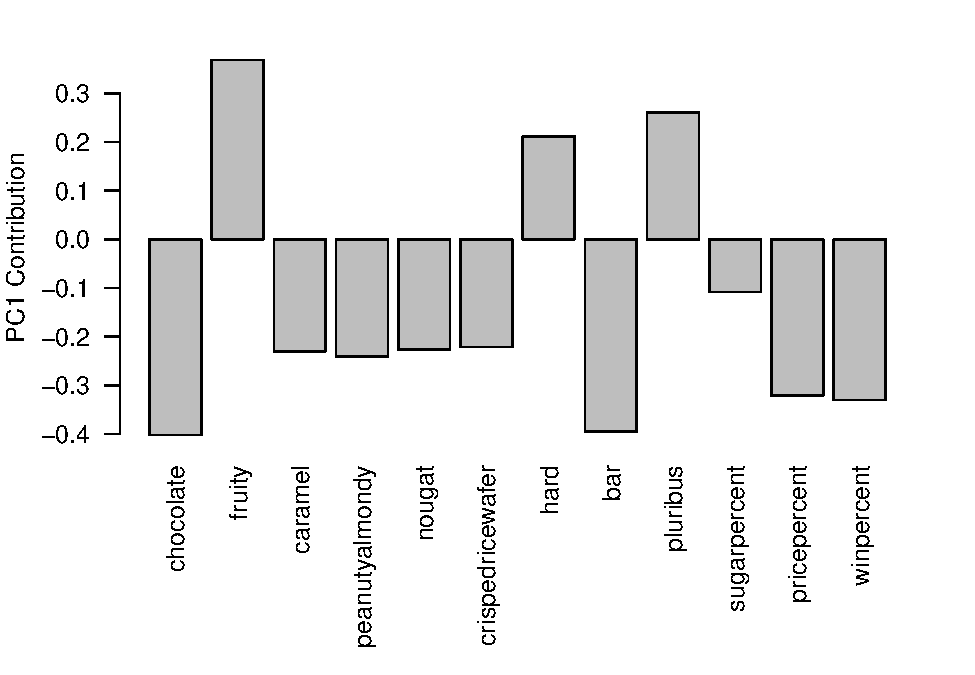
\includegraphics{class17_files/figure-latex/unnamed-chunk-27-1.pdf}

What about 92037 - UCSD / La Jolla?

\begin{Shaded}
\begin{Highlighting}[]
\NormalTok{ucsd }\OtherTok{\textless{}{-}} \FunctionTok{filter}\NormalTok{(sd, zip\_code\_tabulation\_area }\SpecialCharTok{==} \StringTok{"92037"}\NormalTok{)}
\FunctionTok{head}\NormalTok{(ucsd)}
\end{Highlighting}
\end{Shaded}

\begin{verbatim}
##   as_of_date zip_code_tabulation_area local_health_jurisdiction    county
## 1 2021-01-05                    92037                 San Diego San Diego
## 2 2021-01-12                    92037                 San Diego San Diego
## 3 2021-01-19                    92037                 San Diego San Diego
## 4 2021-01-26                    92037                 San Diego San Diego
## 5 2021-02-02                    92037                 San Diego San Diego
## 6 2021-02-09                    92037                 San Diego San Diego
##   vaccine_equity_metric_quartile                 vem_source
## 1                              4 Healthy Places Index Score
## 2                              4 Healthy Places Index Score
## 3                              4 Healthy Places Index Score
## 4                              4 Healthy Places Index Score
## 5                              4 Healthy Places Index Score
## 6                              4 Healthy Places Index Score
##   age12_plus_population age5_plus_population persons_fully_vaccinated
## 1               33675.6                36144                       44
## 2               33675.6                36144                      470
## 3               33675.6                36144                      730
## 4               33675.6                36144                     1079
## 5               33675.6                36144                     1616
## 6               33675.6                36144                     2222
##   persons_partially_vaccinated percent_of_population_fully_vaccinated
## 1                         1265                               0.001217
## 2                         1565                               0.013004
## 3                         3505                               0.020197
## 4                         6197                               0.029853
## 5                         8388                               0.044710
## 6                         9634                               0.061476
##   percent_of_population_partially_vaccinated
## 1                                   0.034999
## 2                                   0.043299
## 3                                   0.096973
## 4                                   0.171453
## 5                                   0.232072
## 6                                   0.266545
##   percent_of_population_with_1_plus_dose redacted
## 1                               0.036216       No
## 2                               0.056303       No
## 3                               0.117170       No
## 4                               0.201306       No
## 5                               0.276782       No
## 6                               0.328021       No
\end{verbatim}

\hypertarget{time-series-of-vaccination-rate-for-92037}{%
\section{Time series of vaccination rate for
92037}\label{time-series-of-vaccination-rate-for-92037}}

\begin{quote}
Q15. Using ggplot make a graph of the vaccination rate time course for
the 92037 ZIP code area:
\end{quote}

\begin{Shaded}
\begin{Highlighting}[]
\FunctionTok{ggplot}\NormalTok{(ucsd) }\SpecialCharTok{+}
  \FunctionTok{aes}\NormalTok{(as\_of\_date,}
\NormalTok{      percent\_of\_population\_fully\_vaccinated) }\SpecialCharTok{+}
  \FunctionTok{geom\_point}\NormalTok{() }\SpecialCharTok{+}
  \FunctionTok{geom\_line}\NormalTok{(}\AttributeTok{group=}\DecValTok{1}\NormalTok{) }\SpecialCharTok{+}
  \FunctionTok{ylim}\NormalTok{(}\FunctionTok{c}\NormalTok{(}\DecValTok{0}\NormalTok{,}\DecValTok{1}\NormalTok{)) }\SpecialCharTok{+}
  \FunctionTok{labs}\NormalTok{(}\AttributeTok{x=}\StringTok{"Date"}\NormalTok{, }\AttributeTok{y=}\StringTok{"Percent Vaccinated"}\NormalTok{, }\AttributeTok{title=}\StringTok{"Vaccination rates for La Jolla 92037"}\NormalTok{)}
\end{Highlighting}
\end{Shaded}

\includegraphics{class17_files/figure-latex/unnamed-chunk-29-1.pdf}

Let's return to the full dataset and look across every zip code area
with a population at least as large as that of 92037 on as\_of\_date
``2021-11-16''.

\begin{Shaded}
\begin{Highlighting}[]
\CommentTok{\# Subset to all CA areas with a population as large as 92037}
\NormalTok{vax}\FloatTok{.36} \OtherTok{\textless{}{-}} \FunctionTok{filter}\NormalTok{(vax, age5\_plus\_population }\SpecialCharTok{\textgreater{}} \DecValTok{36144} \SpecialCharTok{\&}
\NormalTok{                as\_of\_date }\SpecialCharTok{==} \StringTok{"2021{-}11{-}16"}\NormalTok{)}

\FunctionTok{head}\NormalTok{(vax}\FloatTok{.36}\NormalTok{)}
\end{Highlighting}
\end{Shaded}

\begin{verbatim}
##   as_of_date zip_code_tabulation_area local_health_jurisdiction         county
## 1 2021-11-16                    92833                    Orange         Orange
## 2 2021-11-16                    92234                 Riverside      Riverside
## 3 2021-11-16                    92507                 Riverside      Riverside
## 4 2021-11-16                    92555                 Riverside      Riverside
## 5 2021-11-16                    92345            San Bernardino San Bernardino
## 6 2021-11-16                    91306               Los Angeles    Los Angeles
##   vaccine_equity_metric_quartile                 vem_source
## 1                              3 Healthy Places Index Score
## 2                              1 Healthy Places Index Score
## 3                              1 Healthy Places Index Score
## 4                              2 Healthy Places Index Score
## 5                              1 Healthy Places Index Score
## 6                              2 Healthy Places Index Score
##   age12_plus_population age5_plus_population persons_fully_vaccinated
## 1               43985.4                48623                    34668
## 2               46401.1                51202                    34191
## 3               51432.5                55253                    31704
## 4               36725.7                41446                    23776
## 5               66047.5                75539                    35332
## 6               42671.1                46573                    31858
##   persons_partially_vaccinated percent_of_population_fully_vaccinated
## 1                         3377                               0.712996
## 2                         3966                               0.667767
## 3                         3434                               0.573797
## 4                         2424                               0.573662
## 5                         4428                               0.467732
## 6                         3372                               0.684044
##   percent_of_population_partially_vaccinated
## 1                                   0.069453
## 2                                   0.077458
## 3                                   0.062150
## 4                                   0.058486
## 5                                   0.058619
## 6                                   0.072402
##   percent_of_population_with_1_plus_dose redacted
## 1                               0.782449       No
## 2                               0.745225       No
## 3                               0.635947       No
## 4                               0.632148       No
## 5                               0.526351       No
## 6                               0.756446       No
\end{verbatim}

\begin{quote}
How many unique zip codes have a population as large as 92037?
\end{quote}

\begin{Shaded}
\begin{Highlighting}[]
\FunctionTok{length}\NormalTok{(}\FunctionTok{unique}\NormalTok{(vax}\FloatTok{.36}\SpecialCharTok{$}\NormalTok{percent\_of\_population\_fully\_vaccinated))}
\end{Highlighting}
\end{Shaded}

\begin{verbatim}
## [1] 411
\end{verbatim}

\begin{quote}
Q16. Calculate the mean ``Percent of Population Fully Vaccinated'' for
ZIP code areas with a population as large as 92037 (La Jolla)
as\_of\_date ``2021-11-16''. Add this as a straight horizontal line to
your plot from above with the geom\_hline() function?
\end{quote}

\begin{Shaded}
\begin{Highlighting}[]
\FunctionTok{mean}\NormalTok{(vax}\FloatTok{.36}\SpecialCharTok{$}\NormalTok{percent\_of\_population\_fully\_vaccinated)}
\end{Highlighting}
\end{Shaded}

\begin{verbatim}
## [1] 0.6629812
\end{verbatim}

\begin{Shaded}
\begin{Highlighting}[]
\FunctionTok{ggplot}\NormalTok{(ucsd) }\SpecialCharTok{+}
  \FunctionTok{aes}\NormalTok{(as\_of\_date,}
\NormalTok{      percent\_of\_population\_fully\_vaccinated) }\SpecialCharTok{+}
  \FunctionTok{geom\_point}\NormalTok{() }\SpecialCharTok{+}
  \FunctionTok{geom\_line}\NormalTok{(}\AttributeTok{group=}\DecValTok{1}\NormalTok{) }\SpecialCharTok{+}
  \FunctionTok{ylim}\NormalTok{(}\FunctionTok{c}\NormalTok{(}\DecValTok{0}\NormalTok{,}\DecValTok{1}\NormalTok{)) }\SpecialCharTok{+}
  \FunctionTok{labs}\NormalTok{(}\AttributeTok{x=}\StringTok{"Date"}\NormalTok{, }\AttributeTok{y=}\StringTok{"Percent Vaccinated"}\NormalTok{, }\AttributeTok{title=}\StringTok{"Vaccination rates for La Jolla 92037"}\NormalTok{) }\SpecialCharTok{+}
  \FunctionTok{geom\_hline}\NormalTok{(}\AttributeTok{yintercept =} \FloatTok{0.6629812}\NormalTok{, }\AttributeTok{color=}\StringTok{"red"}\NormalTok{, }\AttributeTok{linetype=}\DecValTok{2}\NormalTok{)}
\end{Highlighting}
\end{Shaded}

\includegraphics{class17_files/figure-latex/unnamed-chunk-33-1.pdf}

\begin{quote}
Q17. What is the 6 number summary (Min, 1st Qu., Median, Mean, 3rd Qu.,
and Max) of the ``Percent of Population Fully Vaccinated'' values for
ZIP code areas with a population as large as 92037 (La Jolla)
as\_of\_date ``2021-11-16''?
\end{quote}

\begin{Shaded}
\begin{Highlighting}[]
\FunctionTok{summary}\NormalTok{(vax}\FloatTok{.36}\SpecialCharTok{$}\NormalTok{percent\_of\_population\_fully\_vaccinated)}
\end{Highlighting}
\end{Shaded}

\begin{verbatim}
##    Min. 1st Qu.  Median    Mean 3rd Qu.    Max. 
##  0.3519  0.5891  0.6649  0.6630  0.7286  1.0000
\end{verbatim}

\begin{quote}
Q18. Using ggplot generate a histogram of this data.
\end{quote}

\begin{Shaded}
\begin{Highlighting}[]
\FunctionTok{ggplot}\NormalTok{(vax}\FloatTok{.36}\NormalTok{) }\SpecialCharTok{+}
  \FunctionTok{aes}\NormalTok{(percent\_of\_population\_fully\_vaccinated) }\SpecialCharTok{+}
  \FunctionTok{geom\_histogram}\NormalTok{() }\SpecialCharTok{+}
  \FunctionTok{labs}\NormalTok{(}\AttributeTok{x=}\StringTok{"Percent Vaccinated"}\NormalTok{, }\AttributeTok{y=}\StringTok{"Count"}\NormalTok{)}
\end{Highlighting}
\end{Shaded}

\begin{verbatim}
## `stat_bin()` using `bins = 30`. Pick better value with `binwidth`.
\end{verbatim}

\includegraphics{class17_files/figure-latex/unnamed-chunk-35-1.pdf}

\begin{quote}
Q19. Is the 92109 and 92040 ZIP code areas above or below the average
value you calculated for all these above?
\end{quote}

92040 is below the average and 92109 is above average.

\begin{Shaded}
\begin{Highlighting}[]
\NormalTok{vax }\SpecialCharTok{\%\textgreater{}\%} \FunctionTok{filter}\NormalTok{(as\_of\_date }\SpecialCharTok{==} \StringTok{"2021{-}11{-}16"}\NormalTok{) }\SpecialCharTok{\%\textgreater{}\%}  
  \FunctionTok{filter}\NormalTok{(zip\_code\_tabulation\_area}\SpecialCharTok{==}\StringTok{"92040"}\NormalTok{) }\SpecialCharTok{\%\textgreater{}\%}
  \FunctionTok{select}\NormalTok{(percent\_of\_population\_fully\_vaccinated)}
\end{Highlighting}
\end{Shaded}

\begin{verbatim}
##   percent_of_population_fully_vaccinated
## 1                               0.520463
\end{verbatim}

\begin{Shaded}
\begin{Highlighting}[]
\NormalTok{vax }\SpecialCharTok{\%\textgreater{}\%} \FunctionTok{filter}\NormalTok{(as\_of\_date }\SpecialCharTok{==} \StringTok{"2021{-}11{-}16"}\NormalTok{) }\SpecialCharTok{\%\textgreater{}\%}  
  \FunctionTok{filter}\NormalTok{(zip\_code\_tabulation\_area}\SpecialCharTok{==}\StringTok{"92109"}\NormalTok{) }\SpecialCharTok{\%\textgreater{}\%}
  \FunctionTok{select}\NormalTok{(percent\_of\_population\_fully\_vaccinated)}
\end{Highlighting}
\end{Shaded}

\begin{verbatim}
##   percent_of_population_fully_vaccinated
## 1                               0.687763
\end{verbatim}

\begin{quote}
Q20. Finally make a time course plot of vaccination progress for all
areas in the full dataset with a age5\_plus\_population \textgreater{}
36144.
\end{quote}

\begin{Shaded}
\begin{Highlighting}[]
\NormalTok{vax.}\FloatTok{36.}\NormalTok{all }\OtherTok{\textless{}{-}} \FunctionTok{filter}\NormalTok{(vax, age5\_plus\_population }\SpecialCharTok{\textgreater{}} \DecValTok{36144}\NormalTok{)}


\FunctionTok{ggplot}\NormalTok{(vax.}\FloatTok{36.}\NormalTok{all) }\SpecialCharTok{+}
  \FunctionTok{aes}\NormalTok{(as\_of\_date,}
\NormalTok{      percent\_of\_population\_fully\_vaccinated, }
      \AttributeTok{group=}\NormalTok{zip\_code\_tabulation\_area) }\SpecialCharTok{+}
  \FunctionTok{geom\_line}\NormalTok{(}\AttributeTok{alpha=}\FloatTok{0.2}\NormalTok{, }\AttributeTok{color=}\StringTok{"blue"}\NormalTok{) }\SpecialCharTok{+}
  \FunctionTok{labs}\NormalTok{(}\AttributeTok{x=}\StringTok{"Date"}\NormalTok{, }\AttributeTok{y=}\StringTok{"Percent Vaccinated"}\NormalTok{,}
       \AttributeTok{title=}\StringTok{"Vaccination rates of California"}\NormalTok{,}
       \AttributeTok{subtitle=}\StringTok{"Only areas with a population above 36k are shown"}\NormalTok{) }\SpecialCharTok{+}
  \FunctionTok{geom\_hline}\NormalTok{(}\AttributeTok{yintercept =} \FloatTok{0.66}\NormalTok{, }\AttributeTok{linetype=}\DecValTok{2}\NormalTok{, }\AttributeTok{col=}\StringTok{"red"}\NormalTok{)}
\end{Highlighting}
\end{Shaded}

\begin{verbatim}
## Warning: Removed 180 row(s) containing missing values (geom_path).
\end{verbatim}

\includegraphics{class17_files/figure-latex/unnamed-chunk-38-1.pdf}

\begin{quote}
Q21. How do you feel about traveling for Thanksgiving and meeting for
in-person class next Week?
\end{quote}

I'm fortunate enough that all of my family is local, so I will not be
traveling far for Thanksgiving, and as long as people are vaccinated and
getting frequent COVID tests if they are traveling far / meeting family
that are, I am fine with in-person class next week. Obviously, I would
wish those that are showing symptoms to stay home.

\end{document}
